\documentclass[a4paper, 12pt]{article}
\usepackage[left=17mm, top=17mm, right=17mm, bottom=0mm, headsep=1em]{geometry} % лист а4, 12 кегль, тип документа - статья
\usepackage[utf8]{inputenc}  % кодировка вводимого текста
\usepackage[english, russian]{babel}  % подключение словарей с переносами англ и рус яз
\usepackage{amssymb, latexsym, amsmath, mathtext, bm, gensymb, amssymb}  % пакеты для работы с мат символами
\usepackage{indentfirst}  %  каждый абзац с красной строки
\setlength{\parindent}{4ex}
\linespread{0.4} % межстрочный интервал
 
\usepackage{graphicx}
\graphicspath{ {./images/} }
\usepackage{float}
\usepackage{wrapfig}

\usepackage{bm}
\usepackage{enumitem}
\usepackage[T2A]{fontenc}

\usepackage{fancyhdr}

\newcommand{\RNum}[1]{\uppercase\expandafter{\romannumeral #1\relax}}

\makeatletter
\AddEnumerateCounter{\asbuk}{\russian@alph}{щ}
\makeatother

\pagestyle{fancy}
\fancyhf{}
\rhead{Саженов Константин Станиславович}
\lhead{Группа М8О-108Б-19}
\chead{Вариант 22}
% \rfoot{Page \thepage}
\setlength{\headheight}{28pt}
% \set

\begin{document}
\section*{Задание \RNum{5}} 
\paragraph{Текст задания} Найти остовное дерево с минимальной суммой длин входящих в него ребер. % 2,8,1,7,6,4,3,2,9,8,4,5,1
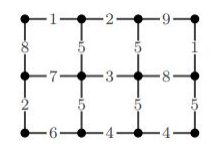
\includegraphics{5_graph}
\begin{enumerate}
    \item Добавляем дуги с весом $1$: $x_3,x_{13}$. Циклов нет
    \item Добавляем дуги с весом $2$: $x_1, x_8$. Циклов нет
    \item Добавляем дуги с весом $3$: $x_7$. Циклов нет
    \item Добавляем дуги с весом $4$: $x_6, x_{11}$. Циклов нет
    \item Добавялем дуги с весом $5$: $x_{16}, x_{12}, x_{15}$. Если добавить ещё $x_{17}$, то будет цикл
    \item Добавляем дуги с весом $6$: $x_5$. Циклов нет. Минимальное остовное дерево построено
\end{enumerate}
$$ L(D) = 1\cdot2 + 2 \cdot 2 + 3 \cdot 1 + 4 \cdot 2 + 5 \cdot 3 + 6 = 38$$
38 - минимальный вес остовного дерева

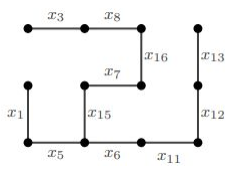
\includegraphics{5_tree}

\end{document}